% Options for packages loaded elsewhere
\PassOptionsToPackage{unicode}{hyperref}
\PassOptionsToPackage{hyphens}{url}
%
\documentclass[
]{article}
\usepackage{amsmath,amssymb}
\usepackage{lmodern}
\usepackage{iftex}
\ifPDFTeX
  \usepackage[T1]{fontenc}
  \usepackage[utf8]{inputenc}
  \usepackage{textcomp} % provide euro and other symbols
\else % if luatex or xetex
  \usepackage{unicode-math}
  \defaultfontfeatures{Scale=MatchLowercase}
  \defaultfontfeatures[\rmfamily]{Ligatures=TeX,Scale=1}
\fi
% Use upquote if available, for straight quotes in verbatim environments
\IfFileExists{upquote.sty}{\usepackage{upquote}}{}
\IfFileExists{microtype.sty}{% use microtype if available
  \usepackage[]{microtype}
  \UseMicrotypeSet[protrusion]{basicmath} % disable protrusion for tt fonts
}{}
\makeatletter
\@ifundefined{KOMAClassName}{% if non-KOMA class
  \IfFileExists{parskip.sty}{%
    \usepackage{parskip}
  }{% else
    \setlength{\parindent}{0pt}
    \setlength{\parskip}{6pt plus 2pt minus 1pt}}
}{% if KOMA class
  \KOMAoptions{parskip=half}}
\makeatother
\usepackage{xcolor}
\usepackage{graphicx}
\makeatletter
\def\maxwidth{\ifdim\Gin@nat@width>\linewidth\linewidth\else\Gin@nat@width\fi}
\def\maxheight{\ifdim\Gin@nat@height>\textheight\textheight\else\Gin@nat@height\fi}
\makeatother
% Scale images if necessary, so that they will not overflow the page
% margins by default, and it is still possible to overwrite the defaults
% using explicit options in \includegraphics[width, height, ...]{}
\setkeys{Gin}{width=\maxwidth,height=\maxheight,keepaspectratio}
% Set default figure placement to htbp
\makeatletter
\def\fps@figure{htbp}
\makeatother
\setlength{\emergencystretch}{3em} % prevent overfull lines
\providecommand{\tightlist}{%
  \setlength{\itemsep}{0pt}\setlength{\parskip}{0pt}}
\setcounter{secnumdepth}{-\maxdimen} % remove section numbering
\ifLuaTeX
  \usepackage{selnolig}  % disable illegal ligatures
\fi
\IfFileExists{bookmark.sty}{\usepackage{bookmark}}{\usepackage{hyperref}}
\IfFileExists{xurl.sty}{\usepackage{xurl}}{} % add URL line breaks if available
\urlstyle{same} % disable monospaced font for URLs
\hypersetup{
  hidelinks,
  pdfcreator={LaTeX via pandoc}}

\author{}
\date{}

\begin{document}

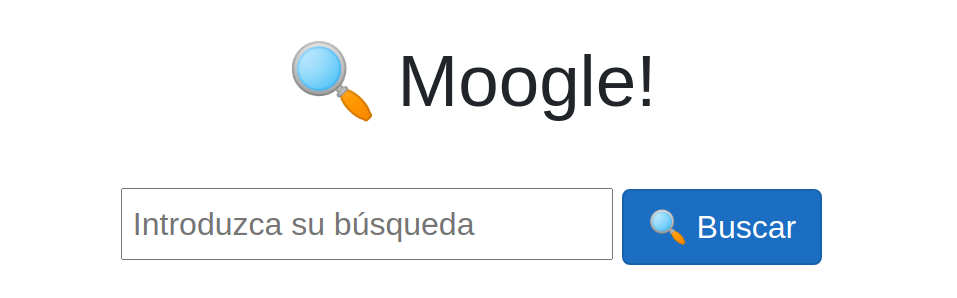
\includegraphics[width=5.90556in,height=1.83889in]{media/image1.png}Moogle!
es una aplicación \emph{*totalmente original*} cuyo propósito es buscar
inteligentemente un texto en un conjunto de documentos. Para tal
propósito se ha empleado el modelo vectorial y el TF-IDF de los términos
para calcular la Similitud Coseno de los documentos y así obtener el
nivel de semejanza entre la query introducida y los documentos.

Clases del Proyecto:

Archivo: Esta clase tiene como objetivo almacenar la información de cada
uno de los documentos de la base de datos.

Propiedades:

//Constante de caracteres separadores.

~ ~ private static char{[}{]} separador=
\{\textquotesingle,\textquotesingle,\textquotesingle.\textquotesingle,\textquotesingle!\textquotesingle,\textquotesingle?\textquotesingle,\textquotesingle;\textquotesingle,\textquotesingle{}
\textquotesingle,\textquotesingle:\textquotesingle,\textquotesingle-\textquotesingle,\textquotesingle*\textquotesingle,\textquotesingle{[}\textquotesingle,\textquotesingle{]}\textquotesingle,\textquotesingle`\textquotesingle,\textquotesingle``\textquotesingle,\textquotesingle''\textquotesingle,\textquotesingle\_\textquotesingle,\textquotesingle(\textquotesingle,\textquotesingle)\textquotesingle,\textquotesingle¿\textquotesingle,\textquotesingle¡\textquotesingle,\textquotesingle/\textquotesingle,\textquotesingle+\textquotesingle,\textquotesingle\#\textquotesingle,\textquotesingle\%\textquotesingle\};

~ ~ //Propiedad que almacena el texto normalizado del documento.

~ ~ public string Texto;

~ ~ //Array de Todas las Palabras del documento.

~ ~ public string{[}{]} Palabras;

~ ~ //Diccionario que almacena Todas las Palabras y la cantidad de veces
que aparecen.

~ ~ public Dictionary\textless string, int\textgreater{} Diccionario =
new Dictionary\textless string, int\textgreater();

~ ~ //Nombre del documento.

~ ~ public string Nombre;

~ ~ //Score que tendrá con respecto a la Query.

~ ~ public double score;

~ ~ //Snippet del documento.

~ ~ public string snippet="";

Métodos:

CrearScore: (Recibe un Diccionario con todas las palabras y sus IDF, y
un diccionario con las palabras de la query y su TF) Calcula el score
del documento por la fórmula:

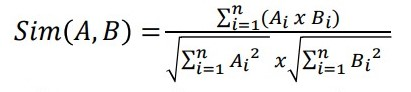
\includegraphics[width=4.28125in,height=0.95833in]{media/image2.png}

CrearSnippet: (Recibe el Diccionario de query) Extrae el snippet
empleando .IndexOf

para determinar la ubicación del término y .Substring para extraer una
porción del texto que lo contenga.

Diccionarios:

Propiedades:

//Propiedad tipo Dictionary que almacena todas las Palabras con un
entero que representa la cantidad de documentos en que aparece.

~ ~ public Dictionary\textless string, int\textgreater{} AllWords;

~ ~ //Propiedad tipo Dictionary que almacena cada palabra con su IDF.

~ ~ public Dictionary\textless string, double\textgreater{} AllWordsIDF;

Métodos:

Incluir: Tiene la función de agregar una palabra al Dictionary AllWords
si la palabra no aparece o sumarle 1 a su Value si aparece.

IDF: Agrega todas las palabras de AllWords a AllWordsIDF y les asigna
como Value su IDF, que se calcula mediante la fórmula:

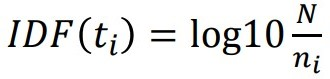
\includegraphics[width=3.4375in,height=0.82292in]{media/image3.png}

Query: Esta clase tiene como objetivo almacenar la query y transformarla
para que sea más fácil efectuar la búsqueda.

Propiedades:

//Propiedad que almacena el texto normalizado de la query.

~ ~ public string Texto;

~ ~ //Array de string con todas las palabras de la query.

~ ~ public string{[}{]} Palabras;

~ ~ //Array de caracteres separadores para hacer Split.

~ ~ private static char{[}{]} separador=
\{\textquotesingle,\textquotesingle,\textquotesingle.\textquotesingle,\textquotesingle!\textquotesingle,\textquotesingle?\textquotesingle,\textquotesingle;\textquotesingle,\textquotesingle{}
\textquotesingle,\textquotesingle:\textquotesingle,\textquotesingle-\textquotesingle,\textquotesingle*\textquotesingle,\textquotesingle{[}\textquotesingle,\textquotesingle{]}\textquotesingle,\textquotesingle`\textquotesingle,\textquotesingle``\textquotesingle,\textquotesingle''\textquotesingle,\textquotesingle\_\textquotesingle,\textquotesingle(\textquotesingle,\textquotesingle)\textquotesingle,\textquotesingle¿\textquotesingle,\textquotesingle¡\textquotesingle,\textquotesingle/\textquotesingle,\textquotesingle+\textquotesingle,\textquotesingle\#\textquotesingle,\textquotesingle\%\textquotesingle\};

~ ~ //Diccionario para almacenar todas las palabras de la query junto
con su TF.

~ ~ public Dictionary\textless string,int\textgreater{} Diccionario =
new Dictionary\textless string, int\textgreater();

~ ~ public double SumatoriaQuery = 0;

Métodos:

CalcularSumatoria: Calcula la sumatoria de los IDF al cuadrado de las
palabras de la query, y lo iguala a la SumatoriaQuery (Este valor nos
será útil más adelante al calcular la similitud coseno.

DataBase: Esta clase es la encargada de cargar y almacenar los valores
necesarios para realizar la búsqueda, por lo que sus propiedades y
métodos serán abordados más adelante en él.

Proceso de Funcionamiento:

Cargar los Documentos: El proceso comienza en MoogleServer, donde justo
antes de iniciar la aplicación se llama al método Load() de la clase
DataBase. Este método obtiene los directorios de los documentos en la
carpeta Content y luego se los envía al constructor de la clase Archivo,
el cual los emplea para obtener el texto de los documentos usando
File.ReadAllText y lo lleva a minúsculas usando .ToLower. Después divide
el texto con .Spit y lo convierte en un array de Palabras que son
agregadas a un Diccionario:

foreach(string palabra in Palabras)

~ ~ ~ ~ \{

~ ~ ~ ~ ~ ~ //Si la palabra ya está se le suma su ocurrencia al TF

~ ~ ~ ~ ~ ~ if(Diccionario.ContainsKey(palabra))

~ ~ ~ ~ ~ ~ \{

~ ~ ~ ~ ~ ~ ~ ~ Diccionario{[}palabra{]}++;

~ ~ ~ ~ ~ ~ \}

~ ~ ~ ~ ~ ~ //Si no está se agrega al Diccionario con ocurrencia 1

~ ~ ~ ~ ~ ~ else

~ ~ ~ ~ ~ ~ \{

~ ~ ~ ~ ~ ~ ~ ~ Diccionario.Add(palabra,1);

~ ~ ~ ~ ~ ~ ~//Método para almacenar todas las Palabras de todos los Doc

~ ~ ~ ~ ~ ~ ~ ~ A.Incluir(palabra);

Tenga en cuenta que se llama al método Incluir por lo que
simultáneamente se van agregando

las palabras a Diccionarios.AllWords. Por último, una vez ya construidos
nuestros objetos tipo Archivo los agregamos a la propiedad estática de
la clase DataBase:

//Propiedad estática que almacena una Lista de objetos de tipo Archivo y
que representa los archivos de la Base de Datos

~ ~ public static List\textless Archivo\textgreater{} Archivos = new
List\textless Archivo\textgreater();

También tenemos la propiedad: public static Diccinarios A = new
Diccinarios();

que gracias al método Incluir posee todas las palabras de la base de
datos de documentos.

Ejecutar Aplicación:

Primero se crea una variable de tipo
List\textless Archivos\textgreater{} de nombre Files y una de tipo
Diccionarios de nombre Words y las igualamos a nuestras propiedades de
la clase DataBase.Archivos y A respectivamente (De esta manera no se
arriesga a modificar la base de datos original). Luego se toma la query
y se crea un objeto tipo Query (la query es enviada al constructor de la
clase Query donde de la misma forma que en la clase Archivo se lleva a
minúsculas su texto y se divide por palabras que son almacenadas en un
Diccionario) y se llama al método CalcularSumatoria para hallar la
SumatoriaQuery, ya con ésta se itera por la Lista Files y se llama al
método CrearScore para hallar el grado de similitud de cada archivo con
la query (score) y de paso se remueven de la Lista usando .Remove todos
los documentos cuyo score es igual a cero. Después se ordena la Lista de
menor a mayor por el score usando:

Files.Sort((o1, o2) =\textgreater{} o1.score.CompareTo(o2.score));

Una vez aplicado este método se emplea el método CrearSnippet sobre los
3 últimos elementos de la Lista Files y se crea una nueva instancia de
la clase SearchItem llamada items con un Length de 3 elementos. Por
último, se agregan el snippet, el Nombre y el score de los 3 últimos
elementos de Files a items y devolvemos items como resultado de nuestra
búsqueda.

\end{document}
